\section{Objectives} 
\label{sec:objectives} 
 
 
The objective of this thesis is to present and implement a generic architectural framework whose intent is to provide an indoor location and satisfy the indoor requirements presented in \ref{sec:int_motivation}. A system implemented on this framework should be capable of keeping its energetic consumption to a minimum and allowing itself to be scalable, deployed in multiple sites and allowing multiple location representations and algorithms. 
 
  
The previously mentioned generic architecture framework can be visualised in figure \ref{fig:solution}. This architecture makes use of the technological developments on mobile phones to use them as the central point of communication of the architecture. This compromise brings onto the table a trade-off where scalability and interoperability are sought in exchange for added communication complexity. On this architecture the beacons are responsible for providing the smartphone information about its surroundings, information that is later on passed onto the location server. This server is responsible for computing the user's location and send it back to him. Once the smartphone is aware of its position, it can request the map server and present the result of the whole process visually to the user. 
 

 \begin{figure}[H] 
\centering 
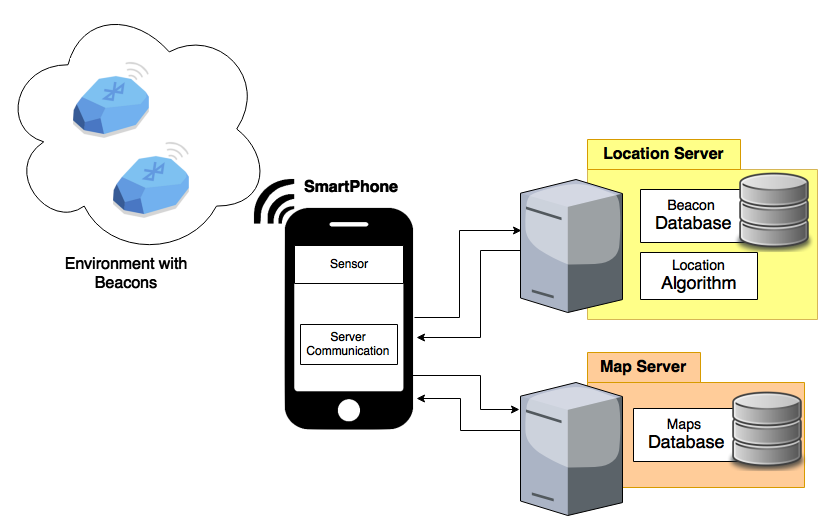
\includegraphics[width=0.7\linewidth]{3.Chapter/generic.png} 
\caption[Generic Architecture Framework]{Generic Architecture Framework } 
\label{fig:solution} 
\end{figure} 
  
 
In order to implement and test the architecture, it was necessary to select the various technologies to use. The chosen technology for the beacons was the Bluetooth low energy, a recent technology that is trying to improve itself in order to be usable on \ac{IoT} and it was capable of providing room-based accuracy without a complex algorithm. The beacon component of the architecture was implemented by making use of \ac{BLE} enabled devices. Each of the devices is uniquely identified and knows the identity of its location server. Whenever a mobile device is nearby one of the beacons, it's capable of establishing a connection with the beacon. This allows it to confirm that the beacon belongs to the indoor location system and to access its data, i.e. the address of the beacon's associated location server. 
 
 
Once the mobile user has all the data from surrounding devices, i.e. he has data associated to the signals collected from each beacon and the address of the server, he can forward it to the location server. The location server has a database with all of its associated devices, that is used to validate the beacon data. Upon confirming that the devices belong to it, it can calculate the user's location through its location algorithm.  
 
 
Upon receiving the user's location, the smartphone is just missing the visual representation of the location. To do so, it sends its location to the map server. The map server in the generic architecture framework represents a server which has a database of all the maps for a certain location server. For this implementation the used map server was google maps since its indoor maps feature was available in the testing place. As such, the location of the mobile user is requested to google maps through its API and presented to the user on its smartphone's screen. 
 
 
The study of the system's energetic costs was created with two questions in mind: What's the impact of the number of nearby beacons? and What are the costs associated to the network communication? The answer to both questions would demonstrate how the overall system performs. 
Since all test results contain the base costs linked to the smartphone, it was vital to start-off by attaining those. Therefore four test were conducted: One with the smartphone inactive (sensors deactivated), two for the Wi-Fi (with and without service) and the last with all sensors active. By making use of these results it would be possible to better comprehend the remaining. 
 
 
For the first question, tests were carried out where two factors were tuned, the number of nearby beacons and the location query's cycle period. From the result's value it was possible to observe the system's high costs. These values are explained by the unoptimised state of the system, evidenced by the fact that the same one/two devices are repeatedly queried for their data in each cycle. In a more optimised solution, the beacon data would be temporarily stored on the smartphone, reducing the costs associated to the \ac{BLE} communication. 
 
 
Meanwhile for the second question, tests were conducted in two different scenarios: One where the system's complete cycle was performed and the other where the cycle was interrupted once the \ac{BLE} communication was finished. Both scenarios were tested with the same amount of nearby beacons and the same cycle period. Through the comparison of both, it was possible to evaluate the impact of the system's network communication, which was fundamental since it consolidated the accepted trade-off for scalability and interoperability. Although the network communication costs aren't negligible, one believes that they are acceptable when taking into consideration the advantages of the proposed architecture.
 